\documentclass{beamer}
\usetheme[block = fill, titleformat title = allcaps, titleformat subtitle  = smallcaps,
progressbar = foot, background = light]{metropolis}           % Use metropolis theme

\usepackage{pgfplots}
\usepackage{appendixnumberbeamer}
\usepackage[font=footnotesize,labelfont=bf]{caption}
\usepackage{booktabs}
\usepackage{amsmath, array}
\usepackage{pifont}
\usepackage{eurosym}

\usetikzlibrary{arrows.meta,positioning, shapes, backgrounds}

\usepackage[sortcites=false,style=authoryear-comp,bibencoding=utf8, natbib=true, firstinits=true, maxcitenames=2, maxbibnames = 99, uniquename=false, backend=bibtex, useprefix=true, backref=false,doi=false,isbn=false,url=false,dashed=true]{biblatex}
\setlength\bibhang{20pt}
\bibliography{../../paper/regions/references.bib}
\AtEveryBibitem{%
	\clearfield{day}%
	\clearfield{month}%
	\clearfield{endday}%
	\clearfield{endmonth}%
}
\AtBeginBibliography{\footnotesize}

\makeatletter
\let\save@measuring@true\measuring@true
\def\measuring@true{%
	\save@measuring@true
	\def\beamer@sortzero##1{\beamer@ifnextcharospec{\beamer@sortzeroread{##1}}{}}%
	\def\beamer@sortzeroread##1<##2>{}%
	\def\beamer@finalnospec{}%
}
\makeatother

\title{Urban exodus or rural shrinkage?}
\subtitle{Regional migration and attractiveness in a tight Dutch housing market}
\date{March 17, 2022}
\author{Thomas de Graaff}
\institute{Vrije Universiteit Amsterdam\\Tinbergen Institute Amsterdam}
\begin{document}
\maketitle

\begin{frame}{Urban Exodus?}
	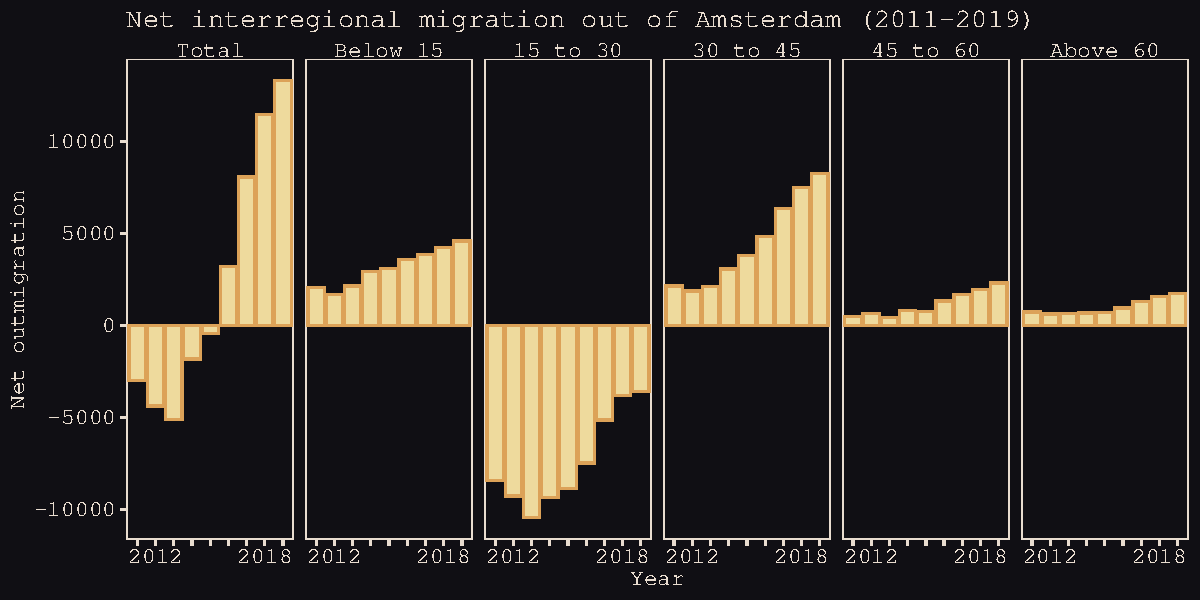
\includegraphics[width=1\textwidth]{../../fig/outmig_amsterdam.pdf}
\end{frame}

\begin{frame}{Dutch population growth 2012--2020}
\begin{columns}
	\begin{column}{0.5\textwidth}
	\begin{itemize}
		\item NUTS-3 regions
		\begin{itemize}
			\item originally (1970) \alert{labour market} regions \newline
		\end{itemize}
		\item Last decade:
		\begin{itemize}
			\item homogeneous population growth
			\item \alert{few} peripheral regions decline\newline
		\end{itemize}
		\item Domestic migration
			\begin{itemize}
				\item slightly more \alert{within} regions than \alert{between} 
				\item growth is the \alert{same}
			\end{itemize}
	\end{itemize}
	\end{column}
	\begin{column}{0.5\textwidth}
		\begin{center}
			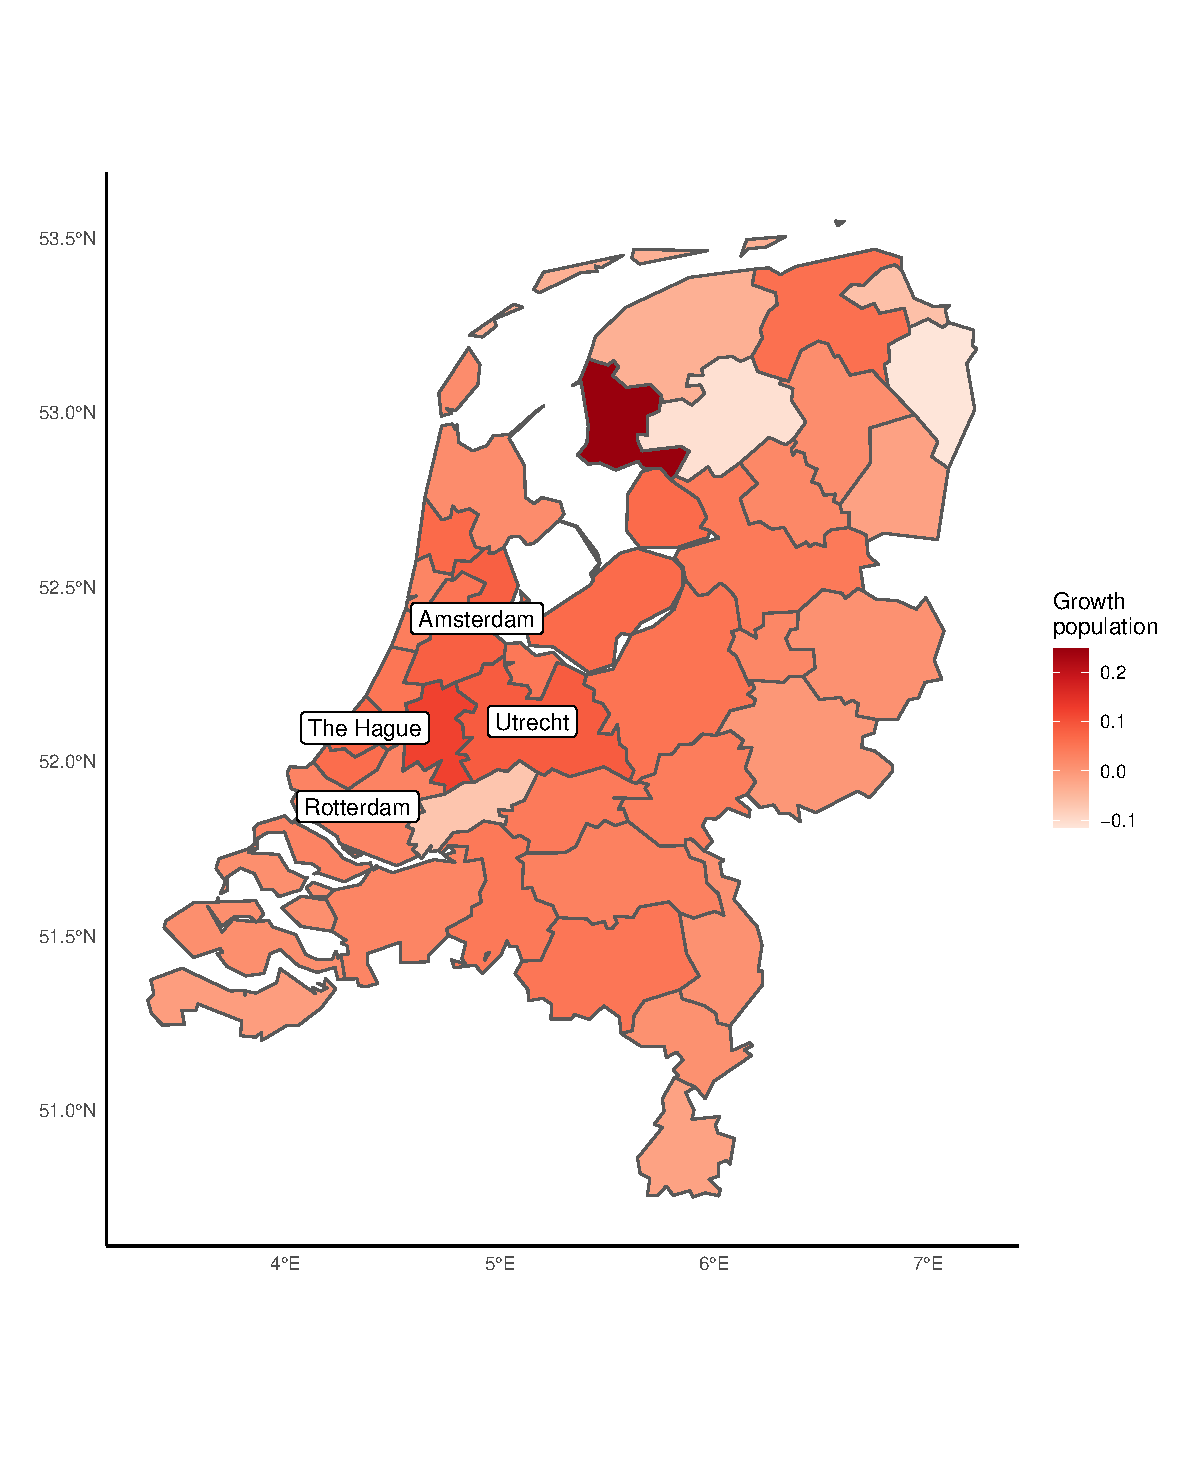
\includegraphics[width=1\textwidth]{../../fig/growth_pop}
		\end{center}
	\end{column}
\end{columns}
\end{frame}

\begin{frame}{\alert{Tight} Dutch housing market}
	\begin{columns}
		\begin{column}{0.5\textwidth}
			\begin{itemize}
				\item Average housing price: \euro 410,000 \newline
				\item Change last year +20\% \newline
				\item \alert{Waiting list} social renting Amsterdam: 13 years \newline
				\item Large \alert{shortage} of housing \newline
				\item Decrease in housing \alert{transactions}
			\end{itemize}
		\end{column}
		\begin{column}{0.5\textwidth}
			\begin{center}
				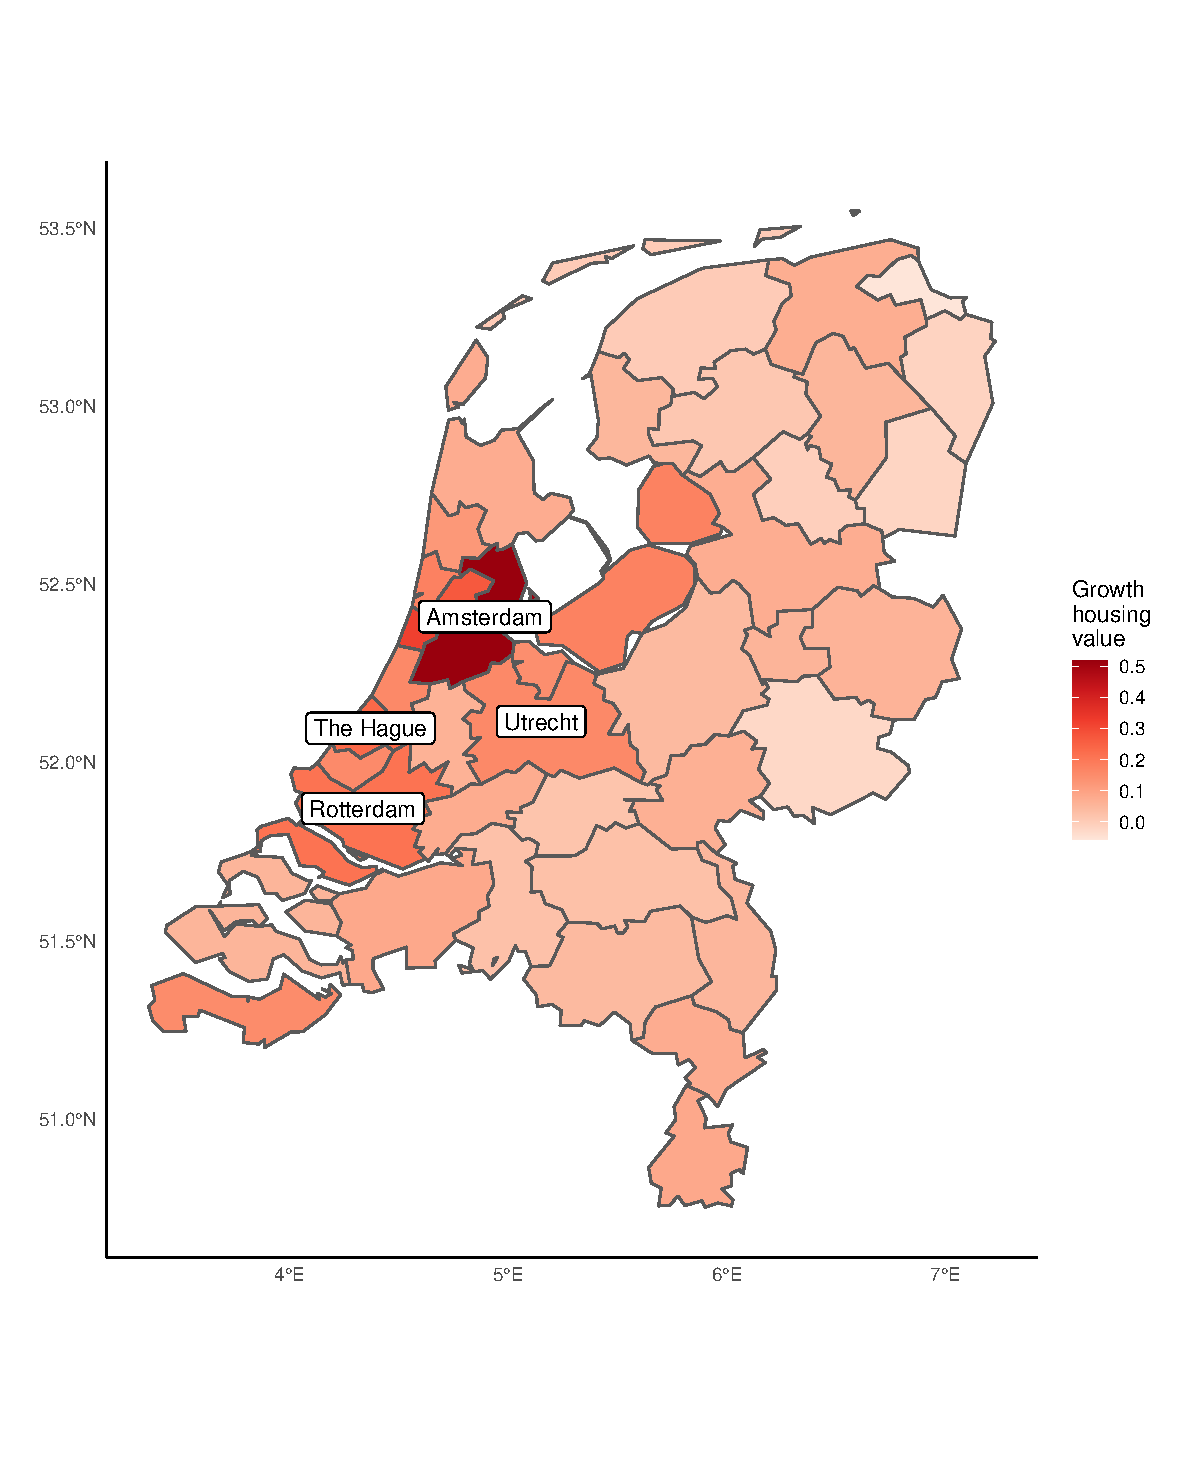
\includegraphics[width=1\textwidth]{../../fig/growth_woz}
			\end{center}
		\end{column}
	\end{columns}
\end{frame}


\begin{frame}{Housing market, urban regions and interregional migration: why bother?}
	Possible \alert{drivers} of urban out-migration?
	  \begin{itemize}
		\item \alert{suburbanisation} of poverty \citep{hochstenbach2018gentrification}
		\item \alert{crowding-out} of the housing market by short-term rentals
		  \citep{koster2021short}
		\item \alert{Influx} of high-skilled migrants
		  \citep{beckers2019residential}
   		\item \alert{Housing market structure} (external effects of home-ownership \citet{dietz2003social})
   		\begin{itemize}
   			\item \alert{negative}: moving costs of home-ownership (and social renting) \citep{oswald1996conjecture,oswald1999housing}
   		\end{itemize}
  \end{itemize}
\end{frame}



\begin{frame}{My contributions to the literature}
  \begin{itemize}
  \item Large empirical (economic) literature on impact housing market structure as driver of interregional migration, but:
    \begin{itemize}
    \item usually focuses on \alert{marginal} effect of home-ownership
    \item less attention for (asymetric) network effects (e.g., push vs. pull effects of larger cities)\newline
    \end{itemize}
  \item Literature on impact of social renting on migration flows is
    scarce \footnotesize{\citep{de2009homeownership} }
	\begin{itemize}
        \item In the Netherlands social renting is a large phenomenon
          ($\approx$ 24\% of total housing stock)
        \item Social renting rights only valid \alert{within} city/region
        \item Social renting is an \alert{urban} phenomenon (e.g. $\approx$
          30--40\% in Amsterdam) 
        \end{itemize}
\end{itemize}
\end{frame}

\begin{frame}{So, this paper}
  \begin{description}
  \item[Does what?] \alert{Estimates} the impact of housing market
	  structure on Dutch interregional migration flows using a
	  \alert{multilevel} gravity model
    \begin{footnotesize}
	\begin{itemize}
	  \item \footnotesize UK context by \citet{congdon2010random}
	  \item \footnotesize \alert{social relations model} \emph{cf.}
		\citet{koster2014food,zhangAnalysingInterprovincialUrban2020}\newline
	\end{itemize}
  \end{footnotesize}
	\item[Aim] To \alert{simultaneously} assess the impact of housing market structure and region specific effects on domestic migration flows
  \begin{footnotesize}
	\begin{itemize}
	  \item \footnotesize home-ownership and social renting
	  \item \footnotesize household size
	  \item \footnotesize percentage western immigrants
	\end{itemize}
  \end{footnotesize}
  \end{description}
\end{frame}


\begin{frame}[fragile]{Why a \alert{multilevel} approach for the gravity model?}
There are at least two \alert{levels} in migration (I use three) \pause
\begin{description}
	\item[Observed migration \alert{flows}] Migration between $i$ and $j$ with friction (e.g., distance) attributes (obs = $R^2 - R$)
		\begin{figure}	
		\begin{tikzpicture}[scale=0.90, thick]
		
		\tikzstyle{orig}=[rectangle, rounded corners, thin, fill=green!20, text=black, draw, minimum width=2cm]
		\tikzstyle{dest}=[rectangle, rounded corners, thin, fill=red!20, text=black, draw, minimum width=2cm]
	\tikzstyle{var}=[rectangle, rounded corners, thin, fill=black!10, text=black, draw, minimum width = 0.6cm, minimum height = 0.4cm]
		\node[orig] (o1) at (0,0)  {\textsc{region$_i$}};
		\node[dest] (d1) at (6,0)  {\textsc{region$_j$}};	
		% Migration links
		\draw[-latex, black, thick] (1.5,0) -- (4.5, 0);
		\node[var] (m) at (3,0)  {\scriptsize \textsc{$\mathbf{X}_{ij}$}};

		\end{tikzpicture}
	\end{figure}\pause
	\item[Observed \alert{push \& pull} factors] Attributes of $i$ and $j$ (obs $= R$)
		\begin{figure}	
	\begin{tikzpicture}[scale=0.90, thick]
	
	\tikzstyle{orig}=[rectangle, rounded corners, thin, fill=green!20, text=black, draw, minimum width=2cm]
	\tikzstyle{dest}=[rectangle, rounded corners, thin, fill=red!20, text=black, draw, minimum width=2cm]
	\tikzstyle{var}=[rectangle, rounded corners, thin, fill=black!10, text=black, draw, minimum width = 0.6cm, minimum height = 0.4cm]
	\node[orig] (o1) at (0,0)  {\textsc{region$_i$}};
	\node[dest] (d1) at (6,0)  {\textsc{region$_j$}};	

	\node[var] (v1) at (0,-1.2)  {\scriptsize \textsc{$\mathbf{X}_i$}};
	\node[var] (v3) at (6,-1.2)  {\scriptsize \textsc{$\mathbf{X}_j$} };

	\draw[-latex, thick, black] (v1) -- (o1);
	\draw[-latex, thick, black] (v3) -- (d1);
	
	\end{tikzpicture}
\end{figure}\pause	
	\item[Observed flows within regional \alert{dyads}] migration from $i \rightarrow j$ is correlated with migration from $j \rightarrow i$ (obs $= \frac{R^{2}- R}{2}$)
			\begin{figure}	
		\begin{tikzpicture}[scale=0.90, thick]
		
		\tikzstyle{orig}=[rectangle, rounded corners, thin, fill=green!20, text=black, draw, minimum width=2cm]
		\tikzstyle{dest}=[rectangle, rounded corners, thin, fill=red!20, text=black, draw, minimum width=2cm]
		\node[orig] (o1) at (0,0)  {\textsc{region$_i$}};
		\node[dest] (d1) at (6,0)  {\textsc{region$_j$}};	
		% Migration links
		\draw[-latex, black, thick] (1.5,0.15) -- (4.5, 0.15);
		\draw[-latex, black, thick] (4.5,-0.15) -- (1.5, -0.15);		
		
		\end{tikzpicture}
	\end{figure}
\end{description}
\end{frame}

\begin{frame}{Why a \alert{Bayesian} multilevel approach?}
\begin{itemize}
	\item Hierarchical, mixed effects, varying intercept/parameter, shrinkage, partial pooling models\pause
	\item Increasingly used for model \alert{performance} and \alert{flexibility} \pause
    \item \alert{Simultaneous} modeling at various levels (e.g., cities, regions, flows, individuals) 
    \begin{itemize}
    	\item no two-stage models anymore 
    	\item precision (standard errors) is correct \alert{at all levels}\pause
    \end{itemize}
	\item \alert{Partial pooling}: For example, origin specific effects are drawn from a distribution: $o_{i} \sim  \mathcal{N}(0, \sigma)$
	\begin{itemize}
		\item $\sigma \longrightarrow 0$ : complete pooling
		\item $\sigma \longrightarrow \infty$ : no pooling (fixed effects)
	\end{itemize}
\end{itemize}
\end{frame}

\begin{frame}{Data: migrations flows in 2018}
	\begin{center}
		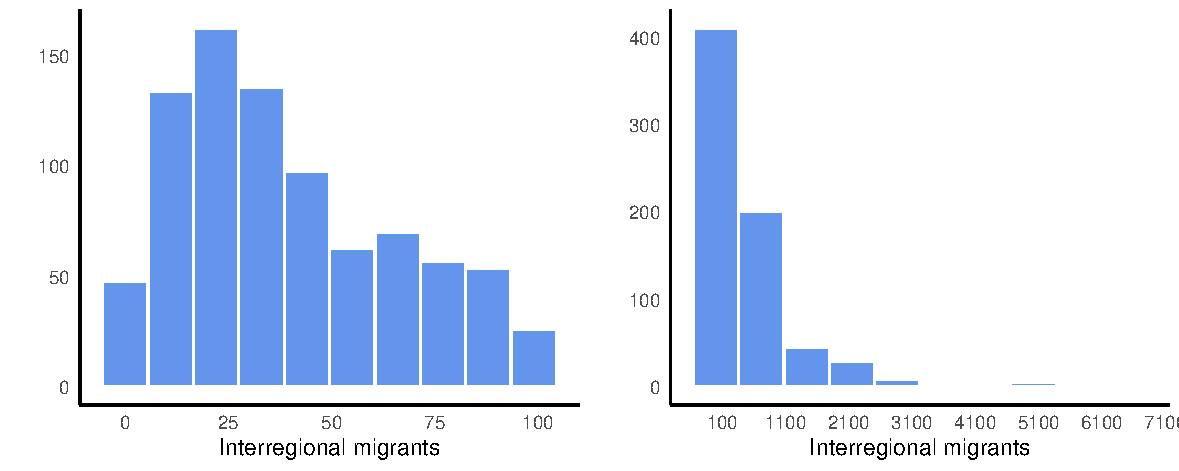
\includegraphics[width=0.8\textwidth]{../../fig/hist_mig_corop}      
	\end{center}
\begin{itemize}
  \item Panel for the period 2012--2020
	\begin{itemize}
		\item estimation: 2012--2019
		\item out-of-sample prediction: 2020
	\end{itemize}
	\item Migration flows \alert{between} 40 Dutch regions
	\item Variance $\gg$ mean: \alert{over-dispersion}
\end{itemize}
\end{frame}

\begin{frame}{Data: regional housing structure in 2018}
\begin{center}
	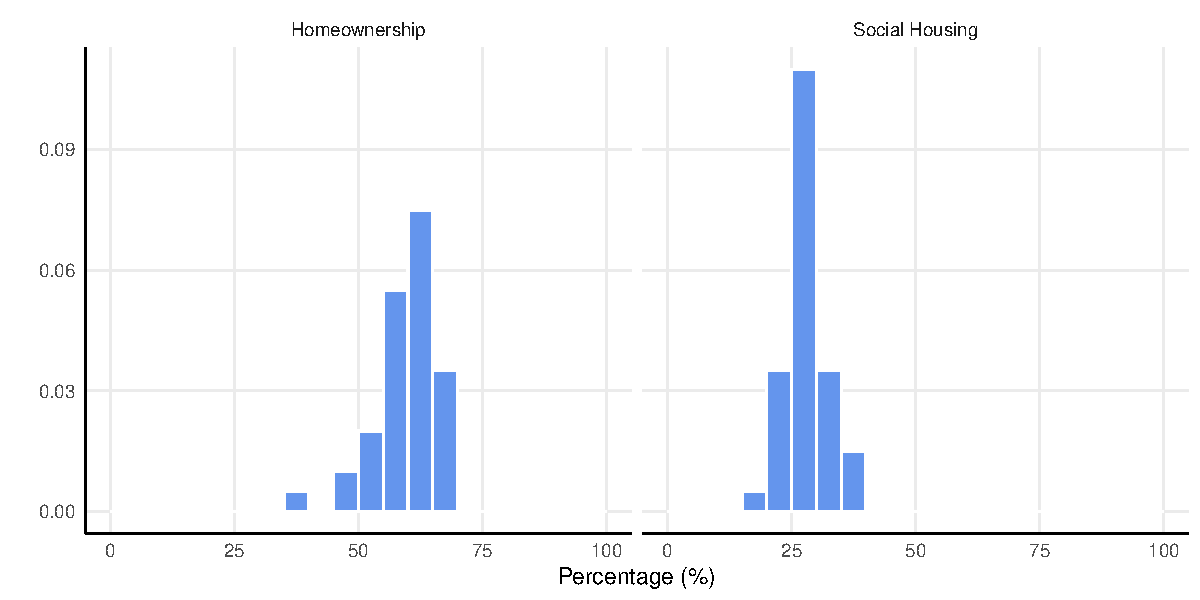
\includegraphics[width=0.8\textwidth]{../../fig/hist_housing_corop}
\end{center}
\begin{itemize}
	\item Positive correlation between regional population and share social renting ($0.46$)
	\item Negative correlation between regional share social renting and share home-ownership ($-0.88)$
\end{itemize}
\end{frame}

\begin{frame}{Data: regional housing structure in 2018 (cont.)}
		\begin{figure}
		  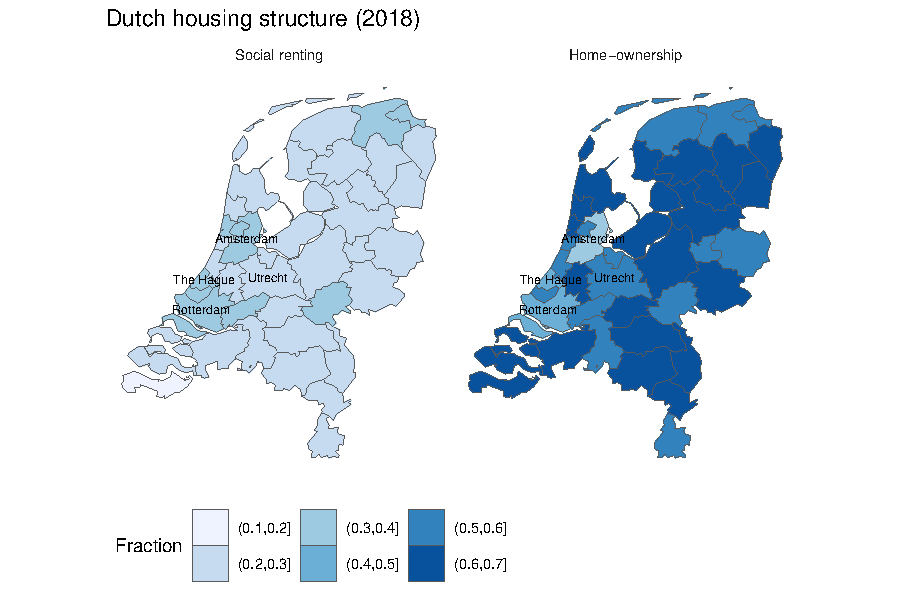
\includegraphics[width=1\textwidth]{../../fig/housing_structure}
		  \end{figure}
\end{frame}

\begin{frame}{Data: regional household size}
	\begin{figure}
		  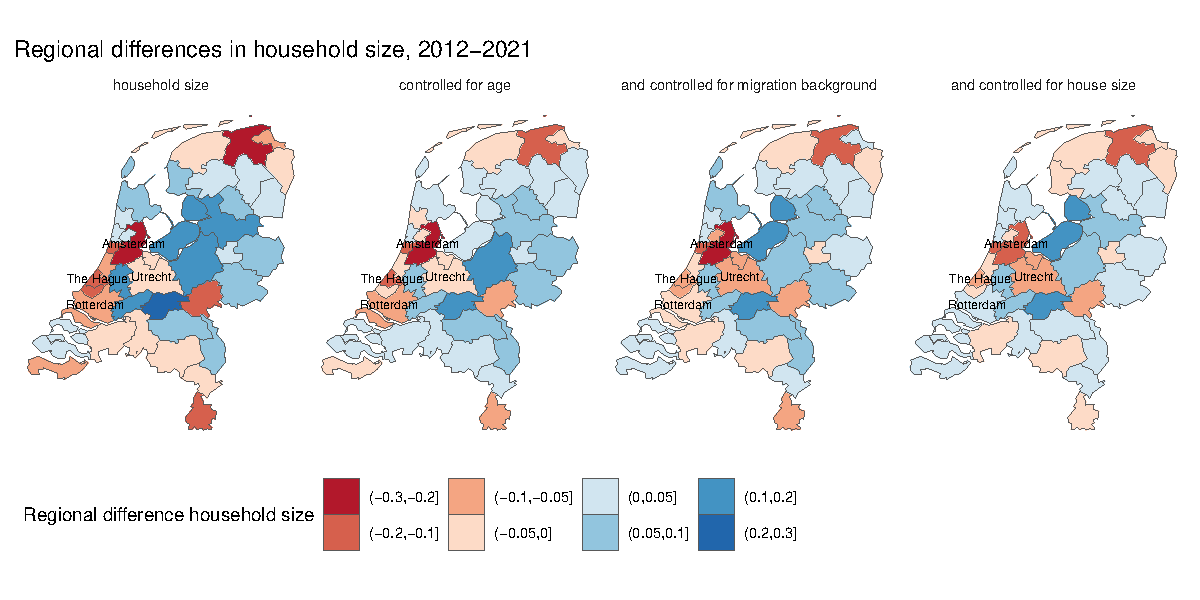
\includegraphics[width=1\textwidth]{../../fig/hhsize_corop}
		  \end{figure}
\end{frame}


\begin{frame}{Modeling framework: traditional gravity modeling}
	\begin{equation*}
	\ln(\text{Migrants}_{ij}) = o_i + d_j + \gamma\ln(\text{dist}_{ij}) + \epsilon_{ij}
	\label{eq:gravfixed}
	\end{equation*} 
	
	Origin and destination specific \alert{regional} effects for multilateral resistance  \citep{anderson2003gravity}, but:
	\begin{itemize}
		\item what about \alert{zeros} in $\text{Migrants}_{ij}$?
		\item how to incorporate \alert{housing} structure in the presence of $o_i$ and $d_j$?
		\item \alert{over-dispersion} and \alert{heteroskedasticity} \footnotesize{\citep{silva2006log} }
	\end{itemize}
\end{frame}

\begin{frame}{Poisson versus negative binomial\footnote{
			\emph{We urge researchers to resist the siren song of the Negative
			Binomial \footnotesize{ \citep{head2014gravity}} }
			}}
	
	\begin{itemize}
		\item \alert{Counts} of migrants\newline 
		\item \alert{Constraints} should hold
		$$
		\sum_{j=1}^{R} {\widehat{\text{Migrants} }_{ij} } = O_i \qquad \sum_{i=1}^{R} {\widehat{\text{Migrants} }_{ij} } = D_j
		$$
		\begin{itemize}
			\item poisson: \ding{51}
		    \item negative binomial: \ding{55} \newline
		  \end{itemize}
		  \item multilevel structure  \alert{controls} for overdispersion
		\end{itemize}

\end{frame}

\begin{frame}[fragile]{Modeling framework: multilevel gravity modeling}
\begin{small}
  \begin{align}
  	\text{Migrants}_{ijt} \sim & \text{Poisson}(\lambda_{ijt})\tag{\footnotesize \color{blue} flow of migrants}\\ \pause
  	\ln(\lambda_{ijt}) = & \alpha +   o_i + d_j + t_t + \text{dyad}_{ij}+ \notag \\
  	& \beta_1 \ln(\text{pop}_{it}) + \beta_2
  	\ln(\text{pop}_{jt}) +
  	\gamma \ln(\text{dist}_{ijt}) + \notag \\
  	& \beta_3 \ln(\text{home}_{it}) +
  	\beta_4 \ln(\text{home}_{jt}) +
  	\beta_5 \ln(\text{soc}_{it}) + \beta_6
	 \ln(\text{soc}_{jt}) + \notag \\
	&  \beta_{7}\ln(\text{hhsize}_{it}) +
	 \beta_{8}\ln(\text{hhsize}_{jt}) + \notag \\
	& \beta_{9}\ln(\text{perc\_wi}_{it}) +
	 \beta_{10}\ln(\text{perc\_wi}_{jt})
	 \tag{\footnotesize \color{blue} linear model} \\ \pause
	\begin{pmatrix}o_i\\
	d_j
\end{pmatrix} \sim &\mathcal{N} \left\{\left(\begin{array}{c}
	0\\
	0
\end{array}\right),
\left(                                        
\begin{array}{cc}
	\sigma^2_i & \rho_{ij} \\
	\rho_{ij} & \sigma^2_{j} 
\end{array}
\right)
\right\} \tag{\footnotesize \color{blue} regional varying effects} \\ \pause
	\begin{pmatrix}\text{dyad}_{ij}\\
	\text{dyad}_{ji}
\end{pmatrix} \sim & \mathcal{N} \left\{\left(\begin{array}{c}
	0\\
	0
\end{array}\right),
\left(                                        
\begin{array}{cc}
	\sigma^2_{\text{dyad}} & \rho \\
	\rho & \sigma^2_{\text{dyad}} 
\end{array}
\right)
\right\} \tag{\footnotesize \color{blue} dyad varying effects} 
\end{align}
\end{small}
\end{frame}


\begin{frame}{Main Estimation results}
				\begin{scriptsize}
\begin{tabular*}{\textwidth}{l @{\extracolsep{\fill}} rr}
				\toprule
  parameter &  origin (push)  & destination (pull) \\
  				\midrule
  				ln(population) 				& $\mathbf{-0.10}$ & $\mathbf{0.70}$ \\
				ln(\% homeownership)  			&  $\mathbf{-1.73}$ & $\mathbf{1.37}$  \\
				ln(\% social renting)  			&  $\mathbf{-0.40}$ & $\mathbf{0.99}$  \\
				ln(household size)  			&  $\mathbf{5.46}$ & $\mathbf{-2.35}$  \\
				ln(\% western immigrants)  	&  $\mathbf{-0.14}$ & $-0.01$  \\
				\addlinespace
				intercept  & \multicolumn{2}{c}{$\mathbf{3.89}$} \\
				\addlinespace
				migrants flow: \\
				\hspace{1cm} ln(distance) &  \multicolumn{2}{c}{$ \mathbf{-1.63}$}  \\
				\addlinespace
				standard deviations: \\
				\hspace{1cm} origin & \multicolumn{2}{c}{$\mathbf{0.67}$} \\
  				\hspace{1cm} destination   & \multicolumn{2}{c}{$\mathbf{0.44}$} \\
				\hspace{1cm} dyad    & \multicolumn{2}{c}{$\mathbf{0.39}$} \\
				 \addlinespace
				correlation \\
				\hspace{1cm} origin-destination   & \multicolumn{2}{c}{$\mathbf{0.78}$} \\
				\hspace{1cm} dyad   &  \multicolumn{2}{c}{$\mathbf{0.80}$}  \\
				\bottomrule
			  \end{tabular*}
		\end{scriptsize}
		\tiny{\textbf{Bold:} 89\% credible intervals do not include zero}\\
		\tiny{Samples are drawn using the NUTS sampler from STAN using 4 chains, each with 4,000 iterations and 1,000 warm-up samples}
\end{frame}

\begin{frame}{Out-of-sample prediction for 2020 ($\text{R}^{2} = 0.98$)}
	\begin{center}
		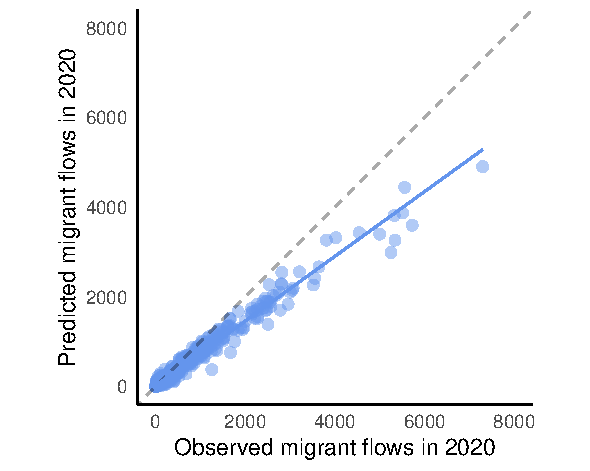
\includegraphics[width=0.9\textwidth]{../../fig/prediction_2020}
	\end{center}
\end{frame}

\begin{frame}{Out-of-sample prediction for 2020 (cntd.)}
	\begin{center}
		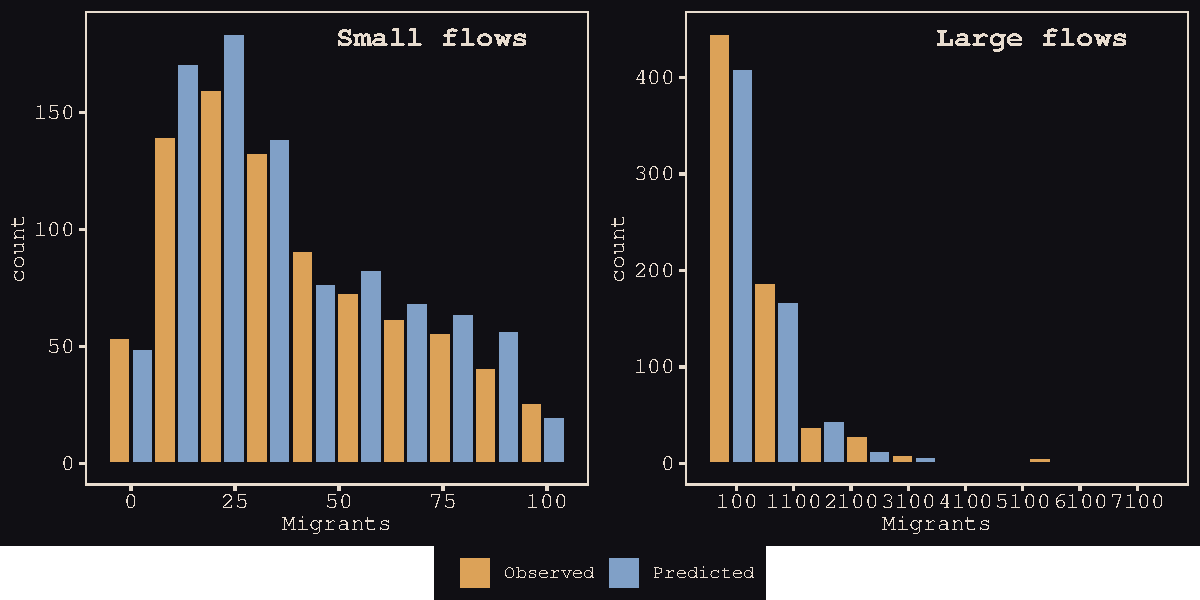
\includegraphics[width=1\textwidth]{../../fig/hist_fit}
	\end{center}
\end{frame}

\begin{frame}{Correlation patterns}
	\begin{center}
		\begin{figure}
			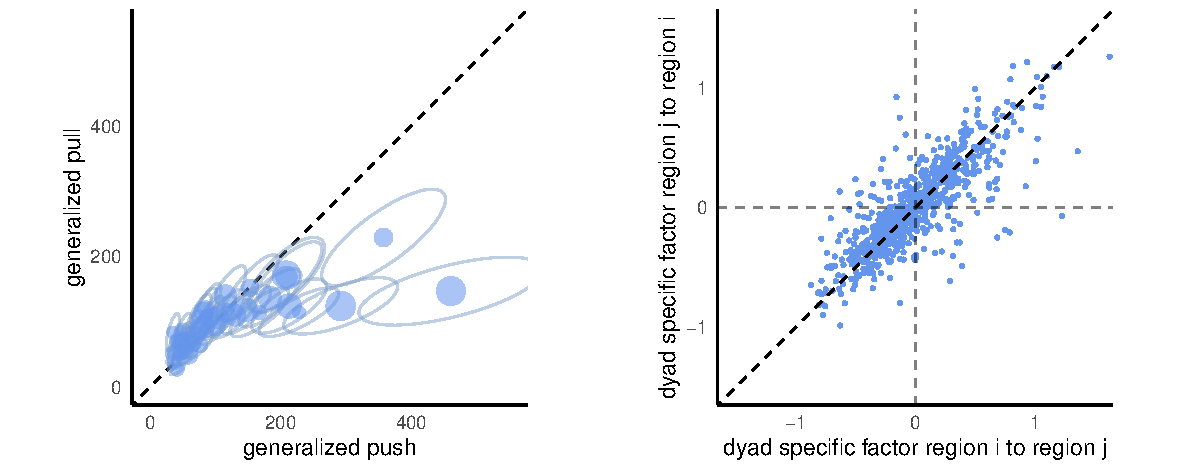
\includegraphics[width=1\textwidth]{../../fig/country_dyad}
			\caption{Correlation (0.78) between unobserved push and pull factors region (left) and flows (correlation = 0.8) within dyad pairs (right)}
		\end{figure}

	\end{center}
\end{frame}


\begin{frame}{Asymmetric push and pull factors}
	\begin{center}
	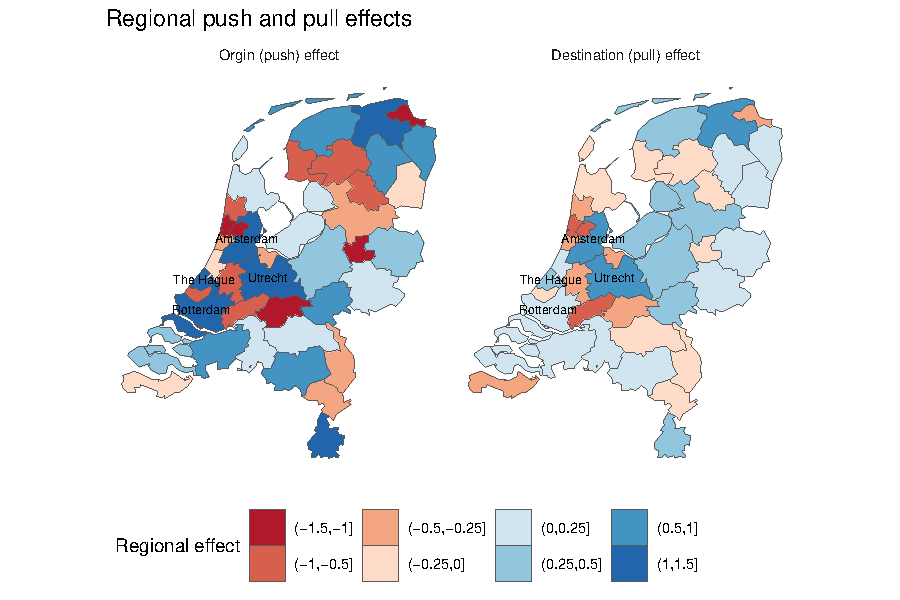
\includegraphics[width=1\textwidth]{../../fig/regional_effects}
\end{center}
\end{frame}

% \begin{frame}{Determinants of push factors?}
% 	\begin{center}
% 		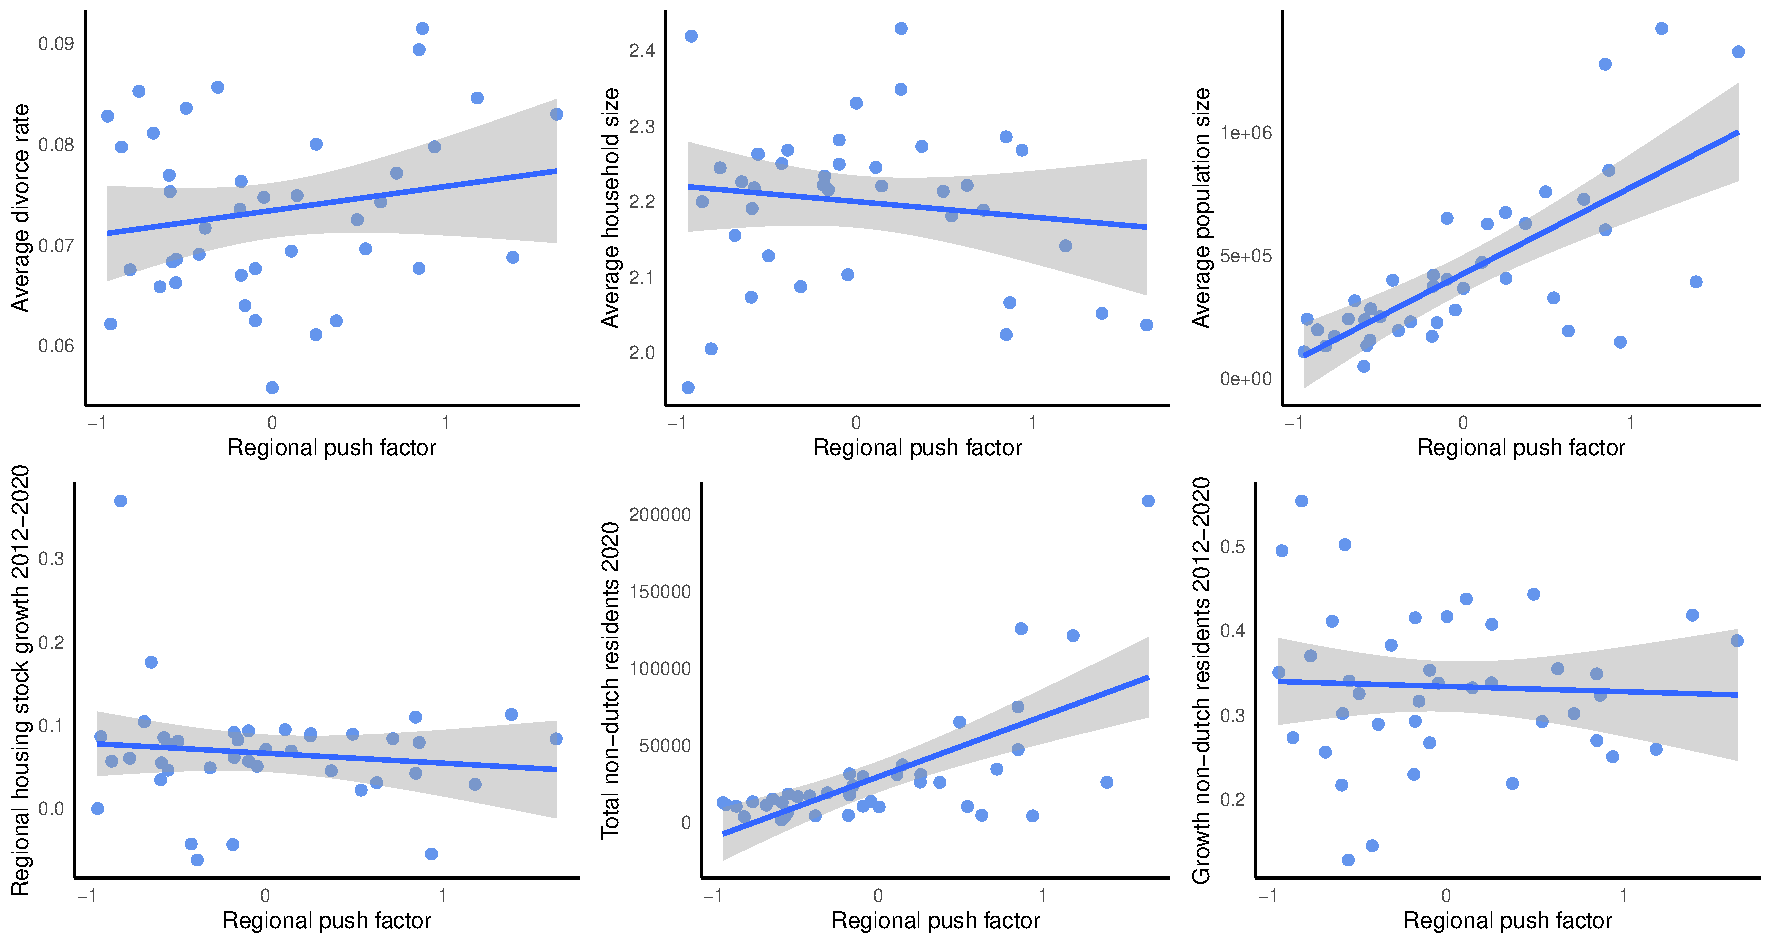
\includegraphics[width=1\textwidth]{../../fig/regional_out_plot}
% 	\end{center}
% \end{frame}

% \begin{frame}{Sensitivity check: temporal stability?}
% 			\begin{center}
% 	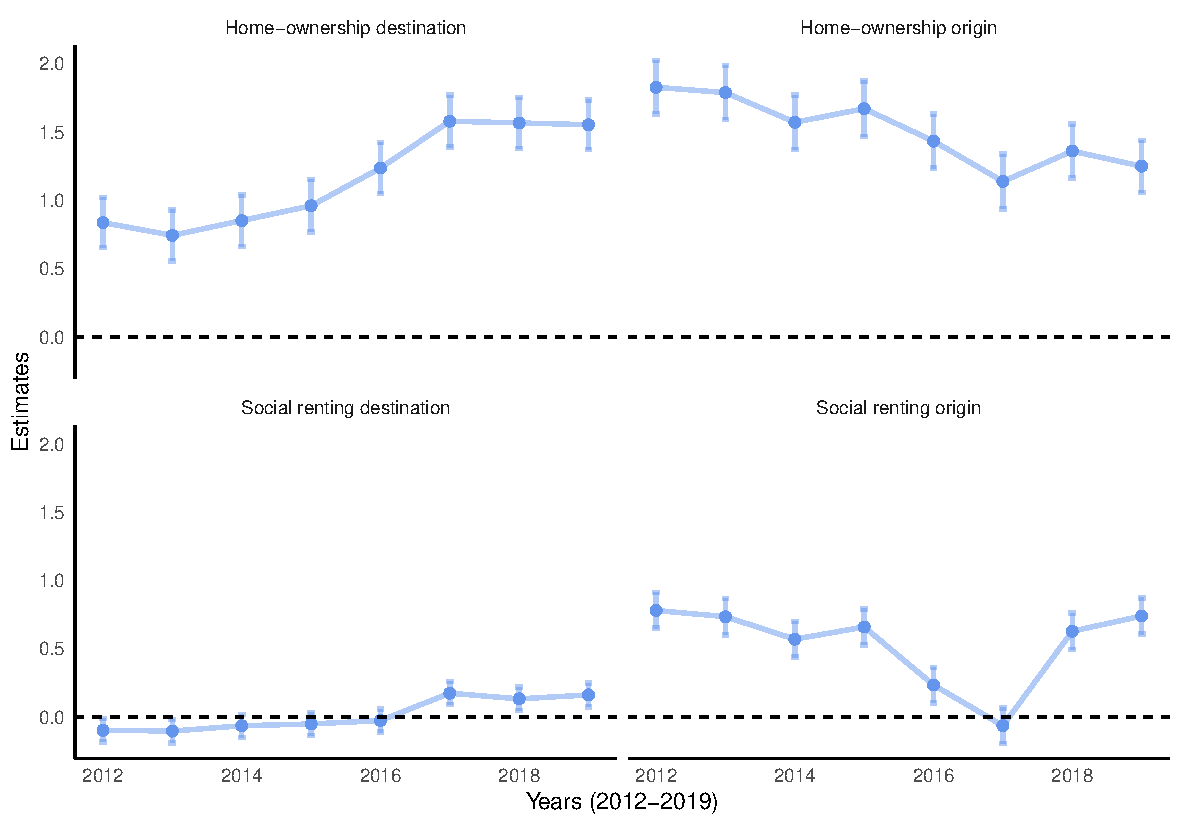
\includegraphics[width=\textwidth]{../../fig/temporal_variation}
% \end{center}
% \
% end{frame}

\begin{frame}{Sensitivity check: spatial autocorrelation}
			\begin{columns}
		\begin{column}{0.5\textwidth}
			\begin{itemize}
				  \item spatial autocorrelation in regional effects:
					\begin{eqnarray*}
					  o_{i}, d_{j}& \sim &\text{MVNormal}(0, \mathbf{K})\\
					  \mathbf{K}_{ij} & = & \eta^{2}\exp(-\rho^{2}\mathbf{D}_{ij}) \newline
					\end{eqnarray*}
					\item results remain robust
					\pause
				  \end{itemize}
		\end{column}
		\begin{column}{0.5\textwidth}
			\alert{Modest} spatial autocorrelation
			\begin{center}
				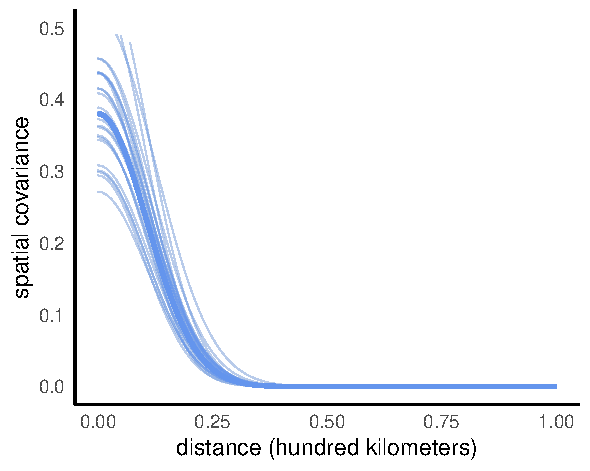
\includegraphics[width=\textwidth]{../../fig/spatial_autocorrelation}
			\end{center}
		\end{column}
	\end{columns}
\end{frame}

\begin{frame}{Conclusions}

\textbf{Main results}:
\begin{itemize}
  \item home-ownership and social renting have \alert{negative} effect on push and \alert{positive} impact on pull factors
  \item household size have \alert{positive} impact on push and \alert{negative} on pull factors
  \item percentage western immigrants small effect
  \item \alert{still} large urban areas have large \alert{push} effects
  \begin{itemize}
	\item effect is different from housing market structure 
	\item more \alert{dynamic} than in periphery
  \end{itemize}
\end{itemize}

\textbf{Speculation}:
\begin{itemize}
 \item \alert{internationalisation}: tourist, short stay (high-skilled), and large housing investment companies drive natives out?
\end{itemize}
\end{frame}

\begin{frame}{Supplementary materials}

Paper, presentation, data and code can be retrieved from the project's GitHub page: 

\begin{center}\url{https://github.com/Thdegraaff/migration\_gravity}\end{center}

\end{frame}

\begin{frame}[standout]
Thank you!
\end{frame}

\appendix

\begin{frame}[allowframebreaks]{References}

		\printbibliography[heading=none]

\end{frame}


\end{document}
